\section{Introduction}



%Often transient simulations are used limited compared to steady state computations as to mitigate the curse of dimensionality that plague particle transport modeling.
%Using more transient

% more general intro problem applications -> Sn transport
Simulating transient particle transport is often required when computing the solution to a number of multi-physics problems, including burst criticality experiments, fission reactor accidents, and other highly dynamic systems.
% Problems to solve and Sn transport
Finding deterministic solutions to the transient neutron transport equation requires some method of treating the contribution of scattering described by an integral.
This is either done by taking moments of the neutron transport equation and making a closure assumption, or by using quadrature to discretize the integral over angle.
The latter is called the method of discrete ordinates (or S$_N$ method, where $N$ is the number of angles in the quadrature) that forms a coupled set of simultaneous PDEs, with one for every direction in a given quadrature set.
The contribution to the scattering source can then be computed using a sum over angles of weights times quantities of interest.
Typically, iterative schemes from operator splitting are used to treat the scattering (and fission) source terms that arise in this coupled set of partial differential equations \cite{lewis_computational_1984}.

% State of the art of transport solvers on CPUs and GPUs warsaw paper, PIDOTS
Source iteration (SI), often accompanied by preconditioners or synthetic accelerators, is a common iteration approach: the contribution to the solution from the scattering source lags, while the angular flux is solved in every ordinate direction via ``sweeps'' through the spatial domain~\cite{adams_subcell_1997}.
SI sweeps in Cartesian geometries readily parallelize over the number of angles.
%The source term is known from the previous iteration, allowing the angular flux in each ordinate to be computed independently.
While any parallelization improves performance, a scheme that is embarrassingly parallel over the dimension with the greatest number of degrees of freedom---space---would be advantageous, especially on vectorized hardware \cite{rosa_cellwise_2013, hoagland_hybrid_2021}.
In a single spatial dimension, SI is ``annoyingly serial'' in space and cannot be parallelized.

In higher spatial dimensions, many S$_N$ production codes that implement SI use a wavefront marching parallel algorithm known as a Koch--Baker--Alcouff scheme \cite{baker_sn_2017}, also called ``full parallel sweeps.''
This algorithm begins a sweep in a spatial location where all cell dependencies are known from boundary information (e.g., a corner).
From there, on a hypothetical orthogonal 2D spatial grid the two nearest neighbor cells are computed independently in parallel; the next step would be across four cells.
This diagonally expanding wavefront continues to march and can compute quantities of interest in parallel for as many cells that lie on the diagonal sweep step.
These sweeps are done on structured or unstructured finite element or finite volume spatial discretization with backward Euler or Crank--Nicholson time stepping iterates.
Source iteration is often solved with preconditioned fixed-point (Richardson) or Krylov sub-space methods (e.g., GMRES) \cite{adams_fast_2002}.
%S$_N$ transport codes that implement this scheme include Partisn \cite{par}, Ardra, Silver Fir, Denovo among others.
%The bulk of modern transport consists preconditioned source iterations sometimes accompanied by GMRES with KBA algorithms in 2D and 3D, FEM/FVM space discretizations, and backward Euler or Crank-Nicholson time stepping.

%When running on GPUs use parallel block domain decomposition with parallel sweeps within the domain. 
%These methods include parallel block Jacobi, inexact parallel block Jacobi, parallel block Gauss-Sidle, and the iterative transport matrix method.
% domain decomptision

%This has proven successful in modern transport applications on CPUs.
%The state of the art in deterministic S$_N$ radiation transport is multi-group in energy distribution, space discretizations or other FEM FVM schemes on unstructured meshes, backward euler time stepping, domain decomposition via parallel block Jacobi, wave front marching schemes like KBA in higher spatial dimensions within a subdomain, and source iterations with diffusion synthetic acceleration (DSA) and potentially accompanied by GMRES solvers. Some examples of production codes that implement this are Partisn, Ardra, Minerate, Capsaicin, Denovo, Silver Fir, etc.

%On CPUs this has been shown to be performant but this changing amount of work is not optimal on GPUs where.
%Performance evaluations of production codes that implement KBA on GPUs is sparse in literature and when available is from proxy-apps.
%Ardra has such a proxy app called Kripkey.
%Kripke is the publicly distributed version of Ardra that has performance data available.
%Roofline models have previously been used to evaluate some miniapps in the Monte Carlo world \cite{tramm2021domain, tramm2022roofline}.
%Roofline analysis of Kripke has been published for performance on an AMD MI200 GPUs \cite{wolfe2022roofline}. 
%Kripley is considered an optimized app yet still cannot land anywhere near the theoretical limits of the GPU hardware.
%We believe this is due to the dynamic work allocation of FPS and think a space parallel scheme would land higher on this chart.

%KBA algorithms are also tricky to efficiently implement in domain decomposed where wave front propagation between boundaries can be tricky.
%While this work is concerned with 1 spatial dimension when analyzing the state of the art it is important to consider that this is done.
%Here again this is included as a
%Each one of these points becomes more difficult to implement due to angle-parallel SI with KBA, for example domain decomposition 

%Published literature on what schemes are implemented, how and their performance on GPU accelerators is sparse.
%Most of my understanding of what is currently used comes from conversations held at conferences with the developers of the codes themselves.
%One place I was able to find performance data on is a mini-app called Kripky \cite{kunen_kripke_2015}.
%Kripke is the publicly distributed version of Ardra that has performance data available.
%Roofline anylisys of Kripke has been published for performance on an AMD MI200 GPUs \cite{wolfe2022roofline}. 
%Specific k
%We conject that this is due to the nonlinear work load a wavefront marching schemes incurred. 

% Intro to OCI and previous work including warsa

%\section{One cell inversions}

An alternative to SI is one-cell inversion (OCI), a class of operator splitting that computes all angular fluxes in all ordinates within a cell in a single linear algebra solve, assuming that the angular fluxes incident on the surfaces of the cell are known from a previous iteration \cite{kang2000oci}.
OCI methods allow parallelizing over the number of cells, as each cell is solved independently in parallel.
OCI iterations can take the form of a cell-wise block-Jacobi, cell-wise block-Gauss--Seidel, or cell-wise red-black iteration depending on the order in which cells are inverted \cite{man1994parallel}.
Like SI, OCI iterations can be fixed-point (Richardson) or non-stationary schemes like GMRES \cite{kylov2004warsa}, with or without preconditioners (including diffusion synthetic acceleration \cite{kang2000oci}) on structured and unstructured meshes.
Parallel block Jacobi and parallel block Gauss--Seidel iterations may also be used for domain decomposition with transport sweeps within subdomains \cite{qiao_improved_2021}.
In fact, OCI methods can be thought of as a cellular decomposed version of these schemes.

\cite{rosa_cellwise_2013} previously studied cell-wise block Jacobi and cell-wise block Gauss--Seidel as a potentially superior iterative scheme over SI preconditioned with diffusion synthetic acceleration on vectorized architectures.
They hypothesized that OCI schemes might outperform an SI preconditioned with diffusion synthetic acceleration and using full-parallel sweeps in terms of wall-clock runtime, because of OCI's parallelism over the dominant domain (space), the ability to take advantage of vendor-supplied LAPACK type libraries, high arithmetic-intensity operations present in an OCI algorithm, and superior spectral properties in the thick limit.
Rosa et al.\ conducted Fourier analysis and implemented OCI in a 2D, multi-group, steady-state code using bilinear discontinuous finite elements to discretize space, a multi-group scheme in energy distribution, and cell-wise block Jacobi and cell-wise block Gauss--Seidel iterations.
The study was conducted on the (then) state-of-the-art RoadRunner supercomputer and took advantage of its 64-bit PowerXCell vectorized accelerator.
However, the acceleration per iteration in the block Gauss--Seidel OCI implementation did not make up for the degradation of convergence that OCI methods incur in the thin limit.
%They concluded by suggesting that future developments in GPU accelerators might overcome this hurtle.

OCI can require more iterations to converge to a solution for some problems, since no information exchanges between cells within an iteration.
Specifically, as cellular optical thickness decreases, OCI's relative performance degrades. %(weather, block Jacobi or block Gauss-Seidel).
Spectral radius ($\rho$) of OCI tends to unity in the thin cell limit---regardless of the scattering ratio---due to the algorithm decoupling cells from one another (i.e., asynchronicity) \cite{rosa_cellwise_2013, hoagland_hybrid_2021, man1994parallel}. 
Figure~\ref{fig:ss-sepcrad} illustrates this behavior, showing the spectral radii of the two iteration schemes as a function of cellular optical thickness, $\delta$ (in mean free paths), and the scattering ratio, $c$.
We compute these values using Fourier analysis of an infinite medium slab problem using S$_{8}$ angular quadrature for block Jacobi OCI and unpreconditioned SI iterative schemes\footnote{Gauss--Legendre quadrature is used in all presented work.}.
The spectral radius of SI depends strongly on the scattering ratio but is independent of $\delta$ for the homogeneous infinite-medium problem. 
Compared to SI, OCI rapidly converges in thicker cells, even in highly scattering problems except for scattering ratios closest to one.

\begin{figure}[htbp]
    \centering
    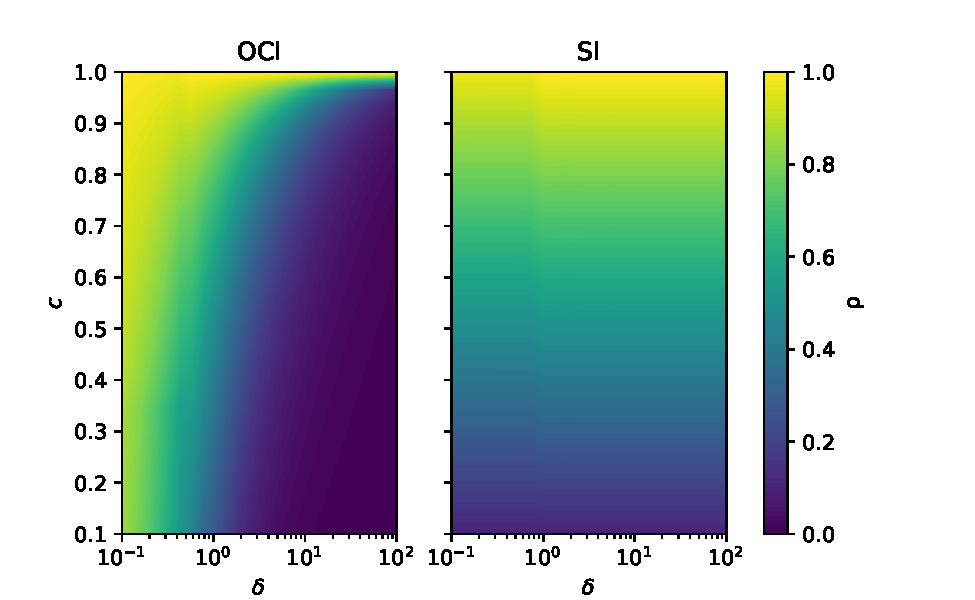
\includegraphics[width=\textwidth]{manuscript2/man2_figs/ss_specrads.pdf}
    \caption{Spectral radii (${\rho}$) of steady-state OCI (left) and SI (right), where $c$ is the scattering ratio and ${\delta}$ is the cellular optical thickness in mean free paths from Fourier analysis in S$_8$.}
    \label{fig:ss-sepcrad}
\end{figure}

Others have explored OCI as an acceleration scheme for SI \cite{ hoagland_hybrid_2021}, a component of a multi-grid solver \cite{man1995multigrid1, man1996multigrid2}, and a solution to the integral transport matrix method \cite{raffi2108pidotscom}.
However, previous investigations of OCI are limited to steady-state computations.

% potential transient effects in the thin limit
When solving initial value problems, Crank--Nicholson, backward Euler, or other time-stepping schemes may be employed.
When implemented, effective time step size ($\Delta t$) and radiation speed ($v$) are inversely proportional to the \textit{effective} total cross section ($\Sigma$).
Returning to Fig.~\ref{fig:ss-sepcrad}, the total cross section ($\Sigma$) influences both the optical thickness of the cell ($\delta$) and the scattering ratio ($c$), so increasing or decreasing $\Sigma$ will impact convergence behavior.
Spectral radius for both iterative methods decreases as the scattering ratio decreases, but \textit{the spectral radius of OCI also decreases with increasing optical thickness}, which in turn depends on $\Sigma$.
When solving optically thin and highly scattering problems, small increases in $\Sigma$ (and for time-dependent problems, decreases in $\Delta t$) may drastically improve the relative performance of OCI compared to SI.
This hypothesis motivates our work, along with evaluating cell-wise algorithms on modern GPU accelerators and exploring higher-order space-time discretization schemes.

% our previous explorations for mono-energetic 1D problems (e.g., many more spatial cells then angles in quadrature)

We previously derived a second-order space (simple corner balance), and time discretization (multiple balance) scheme for block Jacobi OCI (which we will call simply OCI in the remainder of this work) \cite{morgan2023oci}.
We previously showed that when there are more spatial degrees of freedom than in angle, a GPU implementation of OCI will outperform a similarly implemented version of SI in wall clock runtime, in all but the highest scattering problems, for quadrature orders between \num{16} and \num{64} for mono-energetic 1D problems. 

Some derivations from our previous work are included here (Section~\ref{sec:methods-derv}), because we extend it with a Fourier analysis of the discretization scheme through time to ensure it remains unconditionally stable.
We also perform a Fourier analysis on a single time step of OCI and SI to study convergence behaviors in various limits under transient conditions.
Furthermore we extend our derivations to multi-group problems and implement both OCI and SI on an AMD MI250X GPU using vendor-supplied libraries to confirm Fourier results and analyze performance.

